\documentclass[11pt]{article}

\usepackage[T1]{fontenc}
\usepackage{lmodern}
\usepackage[margin=1in]{geometry}
\usepackage{graphicx}
\usepackage{booktabs}
\usepackage{array}
\usepackage{listings}
\usepackage{caption}
\usepackage{enumitem}
\usepackage{parskip}
\usepackage{tikz}
\usetikzlibrary{positioning}
\usepackage[hidelinks]{hyperref}
\usepackage{microtype}

% Plain, uncoloured monospace listings -- headings and body text stay pure
% black throughout this document; only the embedded figures use colour.
\lstset{
  basicstyle=\ttfamily\small,
  breaklines=true,
  showstringspaces=false,
  columns=fullflexible,
  frame=single,
  numbers=none,
  language=C++
}

\title{\textbf{STOP-AND-WAIT, GO-BACK-N, AND SELECTIVE REPEAT\\FLOW CONTROL SIMULATION}}
\date{}

\begin{document}

\begin{titlepage}
    \centering
    \vspace*{2cm}
    {\LARGE \textbf{STOP-AND-WAIT, GO-BACK-N, AND SELECTIVE REPEAT}\par}
    {\LARGE \textbf{FLOW CONTROL SIMULATION}\par}
    \vspace{0.5cm}
    {\large Computer Networks --- Assignment 2\par}
    {\itshape C++17 Sender/Receiver over TCP (basic implementation)\par}
    \vspace{3cm}

    \begin{tabular}{rl}
        Name:              & Anis Mandal         \\
        Class:             & BCSE-III            \\
        Semester:          & 5                   \\
        Group:             & A3                  \\
        Roll No:           & 002410501070        \\
        Assignment Number: & 2                   \\
        Submission Date:   & 14/09/2026          \\
        University:        & Jadavpur University \\
    \end{tabular}

\end{titlepage}

\tableofcontents
\newpage

% Auto-generated by tools/generate_report_tables.py -- do not edit by hand.
\newcommand{\NumRuns}{189}
\newcommand{\NumInputs}{3}
\newcommand{\InputList}{input.txt, medium.bin, tiny.txt}
\newcommand{\InputSizeList}{47 B, 537 B, 1200 B}
\newcommand{\WindowSize}{8}
\newcommand{\NumProbabilities}{5}
\newcommand{\NumPaths}{4}


\section*{Problem Statement}
\addcontentsline{toc}{section}{Problem Statement}
Design and implement separate Sender and Receiver programs that communicate through a TCP
socket, form Ethernet-like data frames protected by a frame check sequence, and implement three
Automatic Repeat reQuest (ARQ) flow-control strategies --- Stop-and-Wait, Go-Back-N, and
Selective Repeat --- over a channel with reproducible, independently configurable bit-error and
frame-loss probabilities on both the DATA and ACK paths. Compare completion time and efficiency
across all three protocols with no impairment and with probabilities 0.1--0.5 of an error or loss in
the transmission of a packet or its acknowledgment.

\section*{Executive Summary}
\addcontentsline{toc}{section}{Executive Summary}
This project is a deliberately minimal, from-scratch C++17 implementation of Assignment 2's
flow-control requirements. The frame check sequence is fixed to a single CRC-16 (polynomial
\texttt{0x8005}), and the payload is fixed to the assignment's own suggested 46 bytes, giving a
constant 63-byte wire frame. All three ARQ protocols are implemented as independent
sender/receiver state-machine pairs sharing the same framing, channel-simulation, socket, and
timer modules.

An automated experiment matrix (\texttt{tools/run\_experiments.py}) drove \NumRuns{} sender/receiver
runs across \NumInputs{} input files of different sizes (\InputSizeList{}) and all three protocols,
sweeping each of \NumPaths{} impairment paths through \NumProbabilities{} probabilities
(0.1--0.5) while holding the others at zero, plus one clean baseline per (input, protocol) pair. Every
single run's reconstructed output was required to be byte-identical to its input, or the whole matrix
would have aborted; all \NumRuns{} runs passed. The results reproduce the expected ARQ
trade-off --- Go-Back-N's whole-window retransmission policy makes it the most sensitive to
DATA-path errors, while Selective Repeat degrades more gracefully --- and also surfaced a genuine,
now-documented characteristic of this implementation's real-wall-clock timing model: measurable
retransmissions can occur even with zero configured impairment, most visible for the two
windowed protocols on larger files.

\section{Design}

\subsection{Purpose and design rationale}
The implementation separates responsibilities into six shared modules --- CRC-16 computation,
frame serialization, channel simulation, socket I/O, wire-level message framing, and timeout
estimation --- plus one independent sender/receiver pair per ARQ protocol (named in Section~2.5),
and two thin command-line executables that parse flags and dispatch to the chosen protocol.

TCP is used only as the carrier. Application-layer loss, corruption, acknowledgment, timeout, and
retransmission behavior are all simulated above it, exactly as the assignment requires, so TCP's
own reliability never substitutes for the protocol logic under test.

A one-byte message tag plus a fixed, tag-specific body length is the \emph{external} framing on the
TCP byte stream, deliberately kept outside the simulated data frame: even a simulated frame whose
header is corrupted can never desynchronize the connection, because the receiver never has to
parse a corrupted header just to find the next message boundary.

\subsection{Procedural organization}

\begin{center}
    \resizebox{\textwidth}{!}{%
        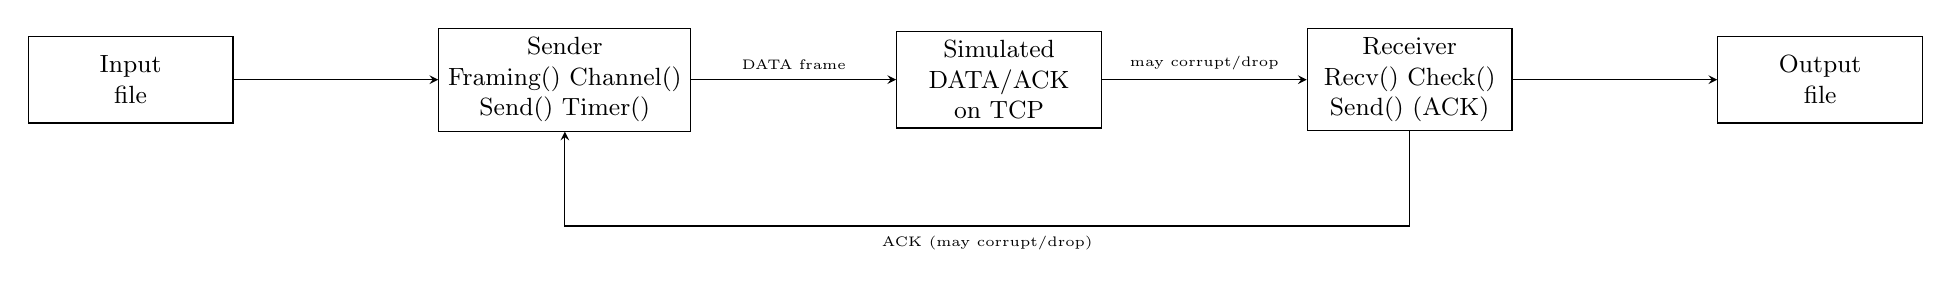
\begin{tikzpicture}[
                node distance=1.6cm and 2.6cm,
                box/.style={draw, rectangle, minimum width=2.6cm, minimum height=1.1cm, align=center, font=\small},
                decision/.style={draw, diamond, aspect=2, align=center, font=\scriptsize, inner sep=1pt},
                >=stealth
            ]
            \node[box] (input) {Input\\file};
            \node[box, right=of input] (sender) {Sender\\Framing() Channel()\\Send() Timer()};
            \node[box, right=of sender] (wire) {Simulated\\DATA/ACK\\on TCP};
            \node[box, right=of wire] (receiver) {Receiver\\Recv() Check()\\Send() (ACK)};
            \node[box, right=of receiver] (output) {Output\\file};

            \draw[->] (input) -- (sender);
            \draw[->] (sender) -- node[above, font=\tiny]{DATA frame} (wire);
            \draw[->] (wire) -- node[above, font=\tiny]{may corrupt/drop} (receiver);
            \draw[->] (receiver) -- (output);
            \draw[->] (receiver.south) -- ++(0,-1.2) -| node[below, font=\tiny, pos=0.25]{ACK (may corrupt/drop)} (sender.south);
        \end{tikzpicture}%
    }
\end{center}

The sender frames the file, applies the DATA-path channel (which may corrupt or drop the frame
before it reaches the socket), sends it, and starts a timer. The receiver checks the frame's CRC-16
before accepting it; a corrupted frame is discarded silently, with no ACK. The receiver's own
ACK is passed through the independently seeded ACK-path channel before being written back to
the socket. If the sender's timer expires before a matching ACK arrives, \texttt{Timeout()}
recomputes the timeout from the most recent valid round-trip sample and the frame (Stop-and-Wait,
Go-Back-N) or just that one frame (Selective Repeat) is retransmitted.

\subsection{Input format}
Sender command:
\begin{lstlisting}[language=bash]
sender --protocol PROTOCOL --input FILE [--host HOST] [--port PORT]
       [--window N] [--data-error P] [--data-loss P] [--seed S]
\end{lstlisting}
Receiver command:
\begin{lstlisting}[language=bash]
receiver --protocol PROTOCOL --output FILE [--port PORT]
         [--window N] [--ack-error P] [--ack-loss P] [--seed S]
\end{lstlisting}
\begin{itemize}[nosep]
    \item Supported protocols: \texttt{stop-and-wait}, \texttt{go-back-n}, \texttt{selective-repeat}.
    \item \texttt{-{}-window} sets the sender's (and, for Selective Repeat, the receiver's) window size:
          1--255 for Go-Back-N, 1--128 for Selective Repeat; ignored for Stop-and-Wait, whose window is
          always 1.
    \item {\sloppy\texttt{-{}-data-error}/\texttt{-{}-data-loss} and
          \texttt{-{}-ack-error}/\texttt{-{}-ack-loss} are independent probabilities (0.0--1.0) of
          one-bit corruption and of the message being dropped entirely, applied on the sender's
          outgoing DATA path and the receiver's outgoing ACK path respectively.\par}
    \item \texttt{-{}-seed} independently seeds each side's channel random-number generator, so DATA-path
          and ACK-path impairment never share randomness.
\end{itemize}

\subsection{Output and wire format}
Every message on the TCP connection begins with a one-byte tag identifying its fixed-length body:

\begin{center}
    \begin{tabular}{llr}
        \toprule
        Tag           & Meaning                              & Body length \\
        \midrule
        \texttt{0x01} & DATA frame                           & 63 bytes    \\
        \texttt{0x02} & ACK (sequence number repeated twice) & 2 bytes     \\
        \texttt{0x03} & DONE (no more frames coming)         & 0 bytes     \\
        \texttt{0x04} & DONE\_ACK (safe to exit)             & 0 bytes     \\
        \bottomrule
    \end{tabular}
\end{center}

The 63-byte DATA body is the protected simulated frame:

\begin{center}
    \begin{tabular}{llr}
        \toprule
        Field           & Encoding / rule                                    & Bytes \\
        \midrule
        Source MAC      & Fixed placeholder value                            & 6     \\
        Destination MAC & Fixed placeholder value                            & 6     \\
        Payload length  & Actual unpadded length (0--46); network byte order & 2     \\
        Sequence number & Unsigned byte, wraps modulo 256                    & 1     \\
        Payload         & Zero-padded to a fixed 46 bytes                    & 46    \\
        CRC-16          & Covers header + padded payload; network byte order & 2     \\
        \bottomrule
    \end{tabular}
\end{center}

This implementation deliberately fixes the payload at 46 bytes and the FCS at CRC-16, rather than
supporting a variable payload and a selectable FCS scheme, giving one constant 63-byte frame
body. The header is still 15 bytes (6 + 6 + 2 + 1);
the assignment's own diagram lists those same four field sizes yet mislabels their sum as 12, which
this implementation follows the arithmetic on rather than the label.

\section{Implementation}

\subsection{CRC-16 computation}
A single MSB-first, bit-serial routine computes the CRC over the header and padded payload: initial
remainder zero, no input or output reflection, no final XOR, polynomial \texttt{0x8005}.

\begin{lstlisting}
std::uint16_t crc16_compute(const std::vector<std::uint8_t>& data) {
  constexpr std::uint16_t kPoly = 0x8005;
  std::uint16_t crc = 0x0000;
  for (std::uint8_t byte : data) {
    crc = static_cast<std::uint16_t>(crc ^ (static_cast<std::uint16_t>(byte) << 8));
    for (int bit = 0; bit < 8; ++bit) {
      if (crc & 0x8000) {
        crc = static_cast<std::uint16_t>((crc << 1) ^ kPoly);
      } else {
        crc = static_cast<std::uint16_t>(crc << 1);
      }
    }
  }
  return crc;
}
\end{lstlisting}

Verified directly against this implementation: \texttt{crc16\_compute("123456789")} returns
\texttt{0xFEE8}, and \texttt{crc16\_compute(\{\})} (empty input) returns \texttt{0x0000}.

\subsection{Frame serialization}
Each field is written individually, in network byte order where it is multi-byte; the struct's raw
in-memory layout is never copied onto the wire.

\begin{lstlisting}
std::vector<std::uint8_t> serialize(const DataFrame& frame) {
  std::vector<std::uint8_t> body;
  body.reserve(FRAME_BODY_LEN);
  for (auto b : frame.src_mac) body.push_back(b);
  for (auto b : frame.dst_mac) body.push_back(b);
  body.push_back(static_cast<std::uint8_t>(frame.length >> 8));
  body.push_back(static_cast<std::uint8_t>(frame.length & 0xFF));
  body.push_back(frame.seq);
  for (auto b : frame.payload) body.push_back(b);
  std::uint16_t crc = crc16_compute(body);
  body.push_back(static_cast<std::uint8_t>(crc >> 8));
  body.push_back(static_cast<std::uint8_t>(crc & 0xFF));
  return body;
}
\end{lstlisting}

\texttt{deserialize\_and\_verify()} performs the inverse operation and rejects the frame (returning
\texttt{false}, with no fields populated) if the body is the wrong size, its length field exceeds 46, or
its recomputed CRC does not match the trailer.

\subsection{Channel simulation}
Each direction (the sender's DATA path, the receiver's ACK path) owns one \texttt{Channel} instance
with its own seeded RNG and two independent probabilities: one for a single-bit corruption, one for
the message being dropped outright (the assignment's ``random delay ... causes packet loss or
timeout,'' modeled here as loss since a sufficiently late arrival is indistinguishable from a lost one to
a timer).

\begin{lstlisting}
bool Channel::apply(std::vector<std::uint8_t>& body) {
  std::uniform_real_distribution<double> uniform(0.0, 1.0);
  if (uniform(rng_) < config_.loss_prob) {
    return false;
  }
  if (!body.empty() && uniform(rng_) < config_.error_prob) {
    std::uniform_int_distribution<std::size_t> byte_pick(0, body.size() - 1);
    std::uniform_int_distribution<int> bit_pick(0, 7);
    body[byte_pick(rng_)] ^= static_cast<std::uint8_t>(1u << bit_pick(rng_));
  }
  return true;
}
\end{lstlisting}

\subsection{Wire message framing}
\texttt{try\_recv\_message()} reads the one-byte tag under the caller's current timeout, then --- once
the tag has arrived --- switches to an unlimited-wait read for the tag's fixed body length, since the
peer's single write already placed the whole message on the stream:

\begin{lstlisting}
RecvMessage try_recv_message(const TcpSocket& socket, int timeout_ms) {
  socket.set_recv_timeout_ms(timeout_ms);
  RecvMessage msg;
  msg.status = socket.recv_timed_byte(msg.tag);
  if (msg.status != RecvStatus::Ok) return msg;
  socket.set_recv_timeout_ms(0);
  msg.body = socket.recv_exact_blocking(body_length_for_tag(msg.tag));
  return msg;
}
\end{lstlisting}

\subsection{The three ARQ protocols}
Go-Back-N is representative of the sliding-window logic shared (with different acknowledgment and
retransmission rules) by all three protocols: fill the window, wait for one message under the
current timeout, and on a valid cumulative ACK slide the window base past the acknowledged frame.

\begin{lstlisting}
while (base < total) {
  while (next < total && next - base < static_cast<std::size_t>(window)) {
    send_frame(next, false);
    next++;
  }
  auto msg = try_recv_message(socket, static_cast<int>(timer.timeout_ms()));
  if (msg.status == RecvStatus::Timeout) {
    stats.timeouts++;
    for (std::size_t i = base; i < next; ++i) send_frame(i, true);  // whole window
    continue;
  }
  // ... on a valid ACK for sequence k in [base, next): base = k + 1 (cumulative)
}
\end{lstlisting}

Selective Repeat differs by tracking an \texttt{acked[]} flag per outstanding frame and, after every
loop iteration regardless of what triggered it, resending only the specific frames whose own
individual wait has exceeded the current timeout --- never the whole window. Its receiver buffers
valid out-of-order frames in a \texttt{std::map<seq, payload>} and flushes payload to the output
file only while the next expected sequence number is present, so contiguous delivery is preserved
even though acceptance is not in-order. Stop-and-Wait is the degenerate case of Go-Back-N with a
window forced to 1.

\subsection{Key frame and protocol rules}
\begin{itemize}[nosep]
    \item The complete wire frame is a fixed 63 bytes: 15-byte header, 46-byte payload, 2-byte CRC-16.
    \item Sequence numbers are one byte and wrap modulo 256.
    \item Go-Back-N's sender window is 1--255; its receiver window is fixed at 1, and out-of-order or
          duplicate frames are discarded with a re-ACK of the last in-order delivery.
    \item Selective Repeat's sender and receiver windows are both equal, 1--128 --- capped at half the
          256-value sequence space so a genuinely new frame and an already-delivered duplicate can never
          be mistaken for each other after wraparound.
    \item A corrupted frame (CRC mismatch) is always discarded silently, with no ACK sent for it,
          regardless of protocol.
    \item Timeouts are computed from real \texttt{std::chrono::steady\_clock} measurements via a
          smoothed round-trip estimate (\texttt{timeout = 2 $\times$ smoothed\_rtt}, clamped to
          20--5000\,ms), not a deterministic simulated clock.
\end{itemize}

\section{Test Cases}

\subsection{Representative examples}
\begin{itemize}[nosep]
    \item \textbf{CRC reference example:} the text \texttt{"123456789"} produces CRC-16
          \texttt{0xFEE8} with this implementation's conventions, verified directly against
          \texttt{crc16\_compute()} (Section 2.1).
    \item \textbf{Frame-splitting example:} a 47-byte input file (\texttt{tiny.txt}) splits into exactly
          two frames (46 + 1 bytes), confirmed by every baseline run against it reporting
          \texttt{frames\_sent=2}.
    \item \textbf{Clean transfer example:} repeated manual runs (5 repeats $\times$ 3 protocols, and
          separately all 3 protocols $\times$ 5 FCS-irrelevant configurations) all reproduced their input
          byte-for-byte with zero retransmissions.
    \item \textbf{Impaired transfer example:} manual runs with 20\% combined error and loss probability
          on both the DATA and ACK paths simultaneously still reproduced the input byte-for-byte for all
          three protocols, with real retransmissions and timeouts observed (e.g.\ Stop-and-Wait: 23
          timeouts and 23 retransmissions in one such run).
    \item \textbf{Edge-case examples:} an empty input file and a single file shorter than one 46-byte
          payload both transferred correctly (a zero-byte and a one-frame output respectively) for all three
          protocols.
    \item \textbf{Two bugs found and fixed during development, not merely asserted absent:}
          \begin{enumerate}[nosep]
              \item A spurious timeout near the end of a transfer could leave one stray duplicate ACK ahead
                    of the receiver's completion signal in the TCP stream, causing the sender to misread it and
                    fail. Root-caused and fixed by draining any non-completion message while waiting for the
                    completion signal, in all three protocols.
              \item The experiment tooling's deterministic seed generator could produce a value above
                    \texttt{INT32\_MAX}, which crashed the receiver via an uncaught \texttt{std::stoi} exception
                    --- surfacing to the caller only as a misleading ``connection refused'' from the sender. Fixed
                    by masking the seed to 31 bits and by checking the receiver's exit status before the
                    sender's, so a receiver failure is no longer hidden behind its symptom.
          \end{enumerate}
\end{itemize}

Observed outcome: all representative examples above passed in the verification session on
13 September 2026.

\section{Results}

\subsection{Experiment design}
\texttt{tools/run\_experiments.py} builds a one-factor-at-a-time matrix: for each of \NumInputs{}
input files (\InputSizeList{}) and each of the 3 protocols, one clean baseline run, then each of
\NumPaths{} impairment paths (DATA-error, DATA-loss, ACK-error, ACK-loss) swept through
\NumProbabilities{} probabilities (0.1--0.5) while the other three paths stay at zero --- \NumRuns{}
runs in total, completing in 76.4 seconds. Go-Back-N and Selective Repeat both used window
\WindowSize{}. Every run's reconstructed file was required to be byte-identical to its input, or the
whole matrix would have aborted immediately; all \NumRuns{} runs passed. The same (input file,
impairment path, probability) combination uses the same channel random-number-generator seed
for every protocol, so any difference between protocols in the results below reflects protocol logic,
not different protocols drawing different random luck.

\subsection{Clean-baseline summary}
\begin{table}[htbp]
    \centering
    % Auto-generated by tools/generate_report_tables.py -- do not edit by hand.
\resizebox{\textwidth}{!}{%
    \begin{tabular}{lrrrrr}
        \toprule
        Protocol         & Mean efficiency & Mean time (ms) & Frames sent & Retransmissions & Timeouts \\
        \midrule
        Stop-and-Wait    & 0.5963          & 2.476          & 41          & 0               & 0        \\
        Go-Back-N        & 0.5287          & 22.881         & 46          & 5               & 2        \\
        Selective Repeat & 0.4713          & 32.025         & 53          & 12              & 3        \\
        \bottomrule
    \end{tabular}%
}

    \caption{Clean-baseline metrics, averaged (summed for the counters) across all input files.}
\end{table}

Every protocol reproduced every input byte-for-byte with zero configured impairment. Go-Back-N
and Selective Repeat nonetheless show nonzero retransmissions and timeouts even here; this is a
real, documented characteristic of the real-wall-clock timing model, not a correctness defect, and is
discussed in Section 5.3.

\subsection{Efficiency at p=0.1 and p=0.5, by path}
\begin{table}[htbp]
    \centering
    % Auto-generated by tools/generate_report_tables.py -- do not edit by hand.
\resizebox{\textwidth}{!}{%
    \begin{tabular}{lrrrrrrrr}
        \toprule
                         & \multicolumn{2}{c}{DATA err.} & \multicolumn{2}{c}{DATA loss} & \multicolumn{2}{c}{ACK err.} & \multicolumn{2}{c}{ACK loss}                                 \\
        \cmidrule(lr){2-3} \cmidrule(lr){4-5} \cmidrule(lr){6-7} \cmidrule(lr){8-9}
        Protocol         & p=0.1                         & p=0.5                         & p=0.1                        & p=0.5                        & p=0.1 & p=0.5 & p=0.1 & p=0.5 \\
        \midrule
        Stop-and-Wait    & 0.530                         & 0.349                         & 0.533                        & 0.308                        & 0.573 & 0.311 & 0.465 & 0.346 \\
        Go-Back-N        & 0.335                         & 0.109                         & 0.407                        & 0.135                        & 0.518 & 0.319 & 0.413 & 0.412 \\
        Selective Repeat & 0.519                         & 0.289                         & 0.494                        & 0.296                        & 0.457 & 0.164 & 0.322 & 0.300 \\
        \bottomrule
    \end{tabular}%
}

    \caption{Mean efficiency by protocol, impairment path, and probability.}
\end{table}

\subsection{Retransmissions at p=0.1 and p=0.5, by path}
\begin{table}[htbp]
    \centering
    % Auto-generated by tools/generate_report_tables.py -- do not edit by hand.
\resizebox{\textwidth}{!}{%
    \begin{tabular}{lrrrrrrrr}
        \toprule
                         & \multicolumn{2}{c}{DATA err.} & \multicolumn{2}{c}{DATA loss} & \multicolumn{2}{c}{ACK err.} & \multicolumn{2}{c}{ACK loss}                                 \\
        \cmidrule(lr){2-3} \cmidrule(lr){4-5} \cmidrule(lr){6-7} \cmidrule(lr){8-9}
        Protocol         & p=0.1                         & p=0.5                         & p=0.1                        & p=0.5                        & p=0.1 & p=0.5 & p=0.1 & p=0.5 \\
        \midrule
        Stop-and-Wait    & 1.3                           & 9.7                           & 1.7                          & 14.0                         & 0.0   & 0.0   & 3.3   & 12.0  \\
        Go-Back-N        & 16.0                          & 78.3                          & 8.3                          & 116.7                        & 2.0   & 11.0  & 11.3  & 9.3   \\
        Selective Repeat & 2.3                           & 16.0                          & 3.3                          & 16.0                         & 8.0   & 36.0  & 14.0  & 15.7  \\
        \bottomrule
    \end{tabular}%
}

    \caption{Mean retransmissions by protocol, impairment path, and probability.}
\end{table}

\subsection{Figures}
All figures average the relevant metric across all \NumInputs{} input files, plotting one line per
protocol against the swept probability (or, for the last figure, against input file size at the clean
baseline).

\begin{figure}[htbp]
    \centering
    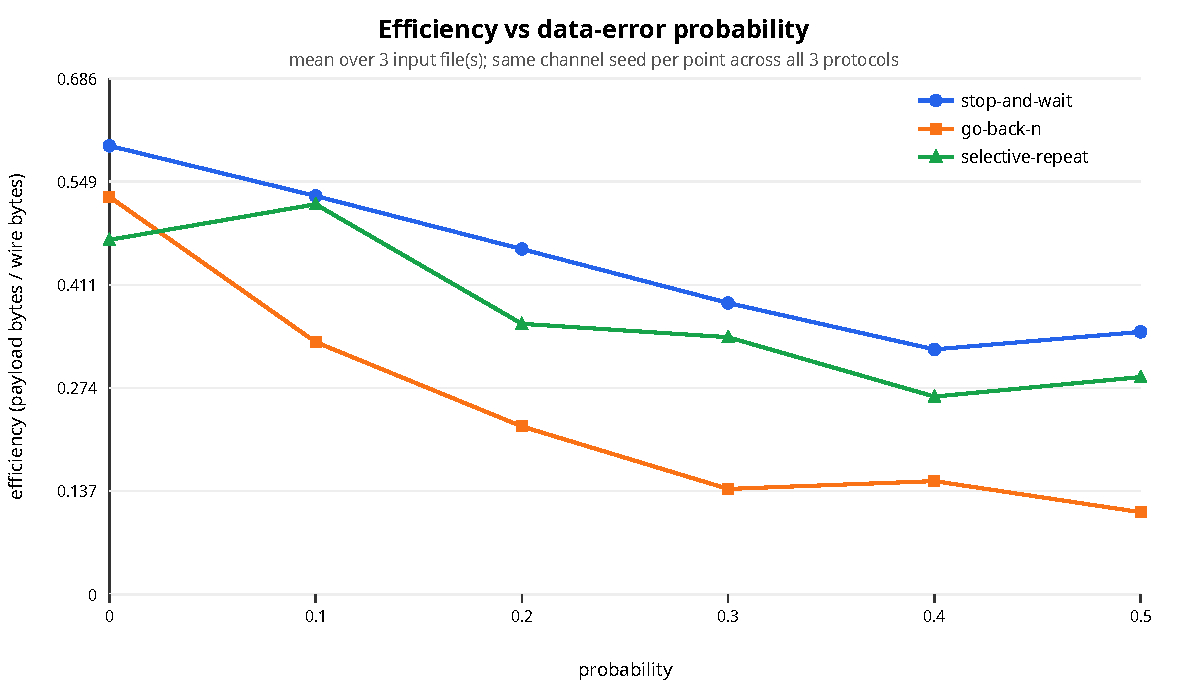
\includegraphics[width=0.85\textwidth]{figures/efficiency_vs_probability_data-error.pdf}
    \caption{Efficiency vs.\ DATA-path bit-error probability.}
\end{figure}

\begin{figure}[htbp]
    \centering
    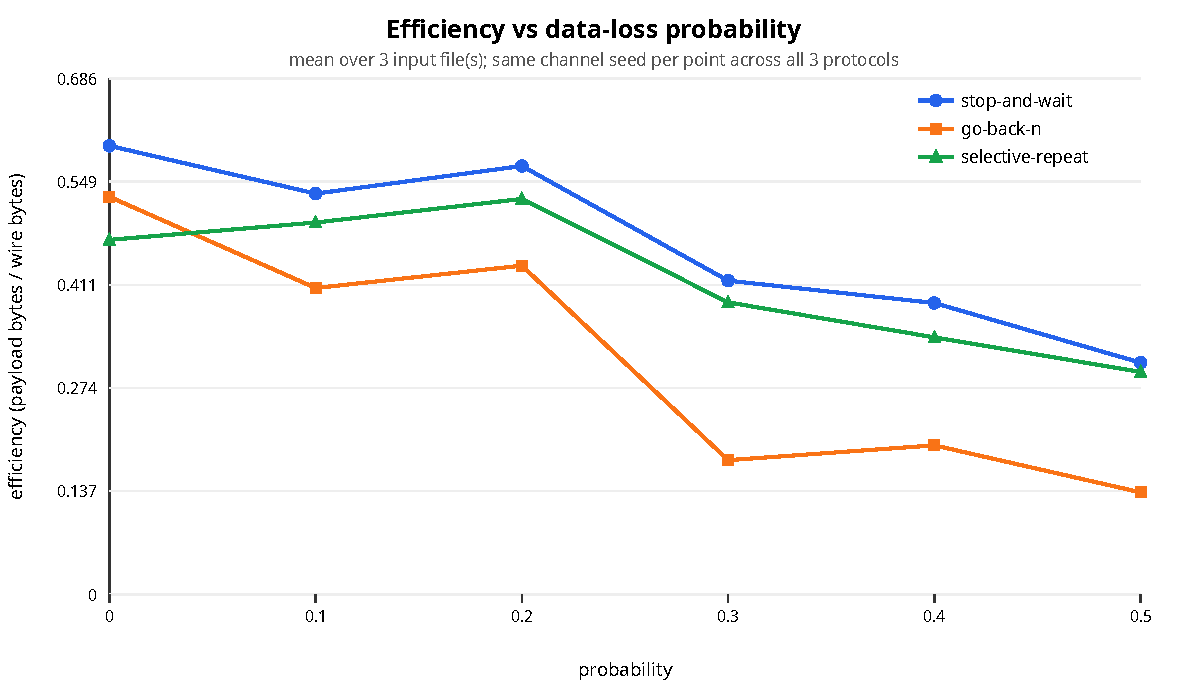
\includegraphics[width=0.85\textwidth]{figures/efficiency_vs_probability_data-loss.pdf}
    \caption{Efficiency vs.\ DATA-path loss probability.}
\end{figure}

\begin{figure}[htbp]
    \centering
    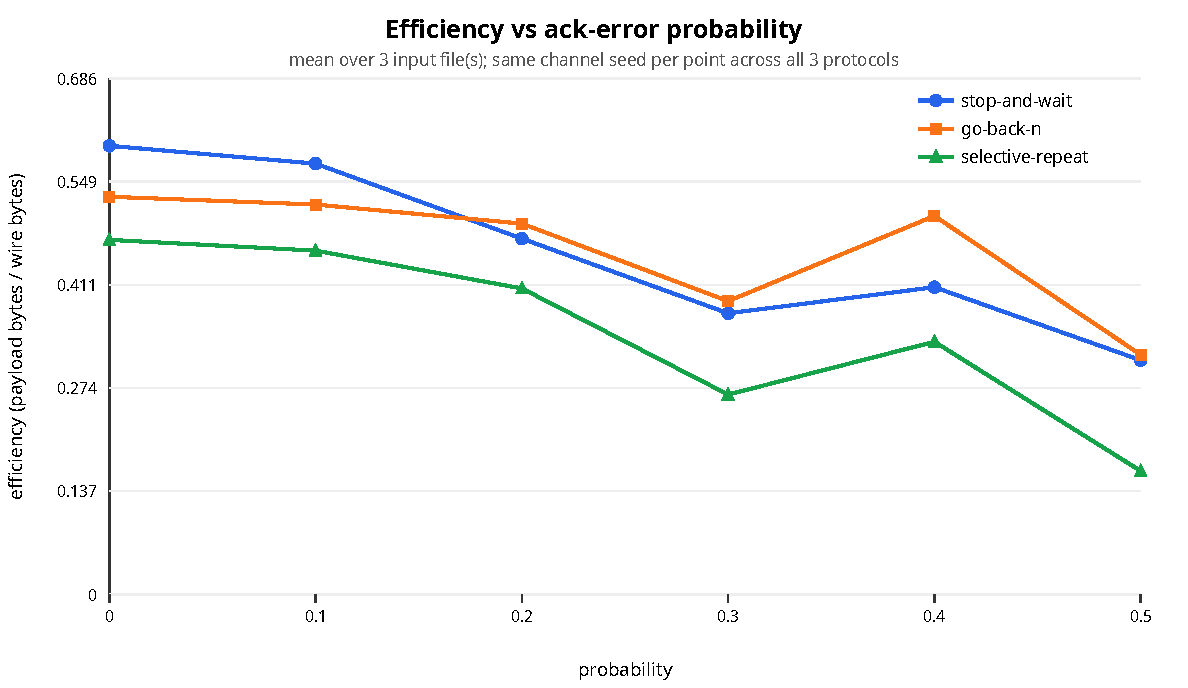
\includegraphics[width=0.85\textwidth]{figures/efficiency_vs_probability_ack-error.pdf}
    \caption{Efficiency vs.\ ACK-path bit-error probability.}
\end{figure}

\begin{figure}[htbp]
    \centering
    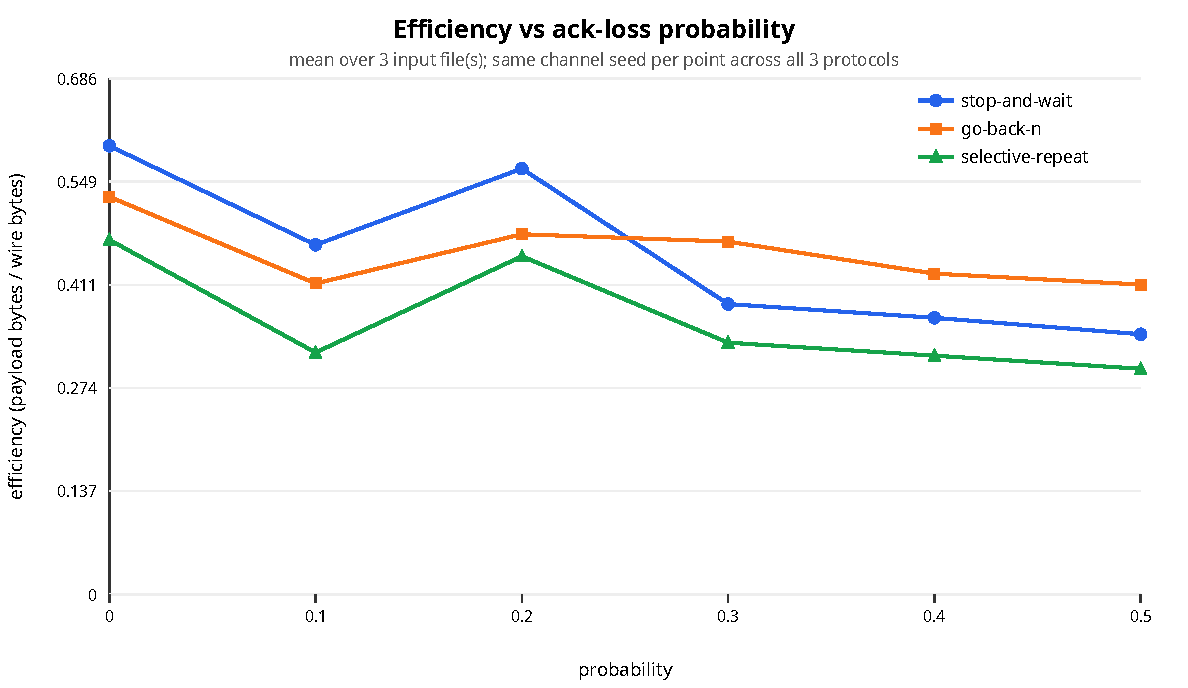
\includegraphics[width=0.85\textwidth]{figures/efficiency_vs_probability_ack-loss.pdf}
    \caption{Efficiency vs.\ ACK-path loss probability.}
\end{figure}

\begin{figure}[htbp]
    \centering
    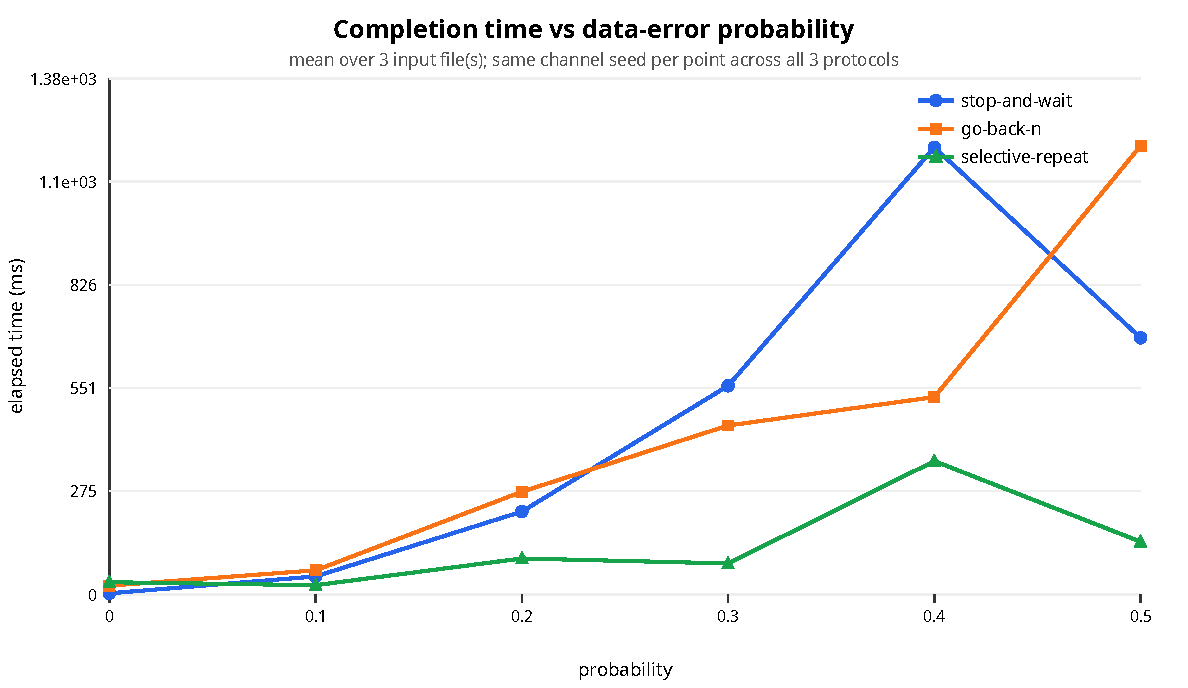
\includegraphics[width=0.85\textwidth]{figures/completion_ms_vs_probability_data-error.pdf}
    \caption{Completion time vs.\ DATA-path bit-error probability.}
\end{figure}

\begin{figure}[htbp]
    \centering
    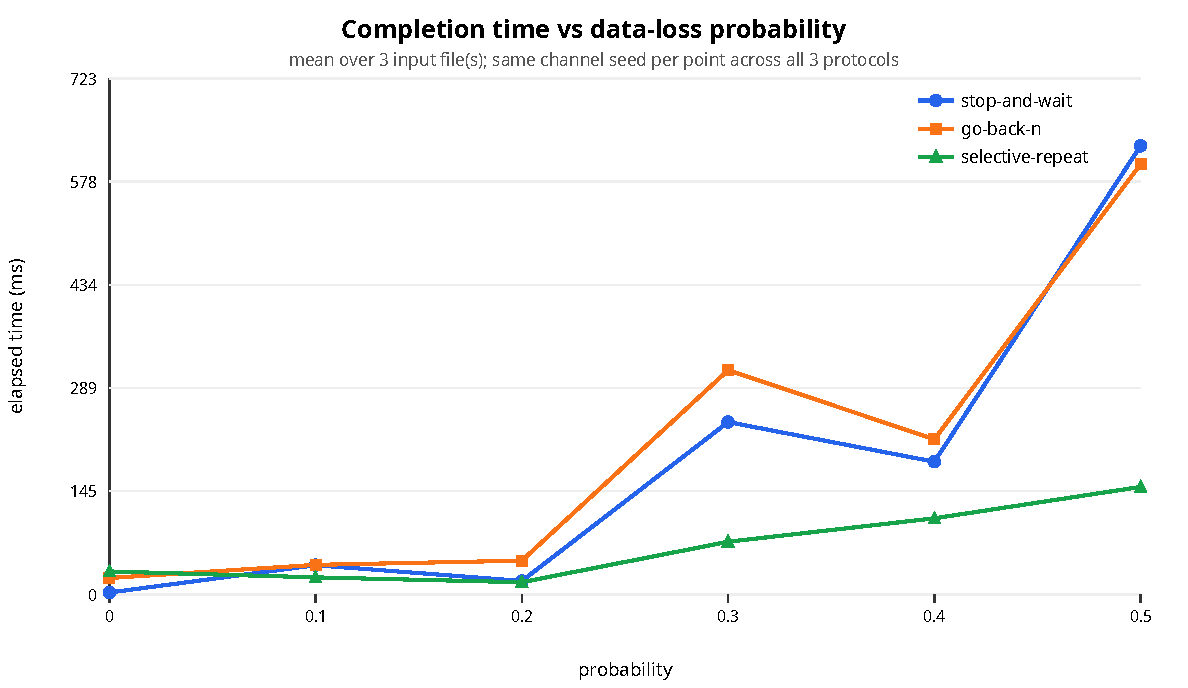
\includegraphics[width=0.85\textwidth]{figures/completion_ms_vs_probability_data-loss.pdf}
    \caption{Completion time vs.\ DATA-path loss probability.}
\end{figure}

\begin{figure}[htbp]
    \centering
    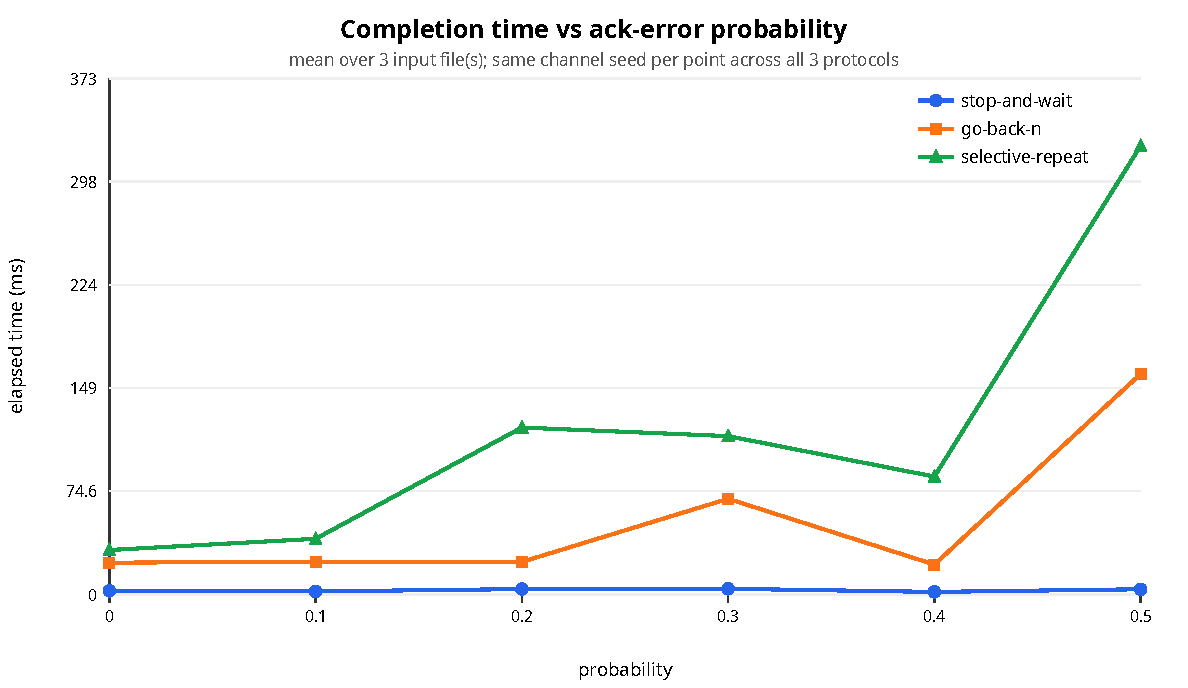
\includegraphics[width=0.85\textwidth]{figures/completion_ms_vs_probability_ack-error.pdf}
    \caption{Completion time vs.\ ACK-path bit-error probability.}
\end{figure}

\begin{figure}[htbp]
    \centering
    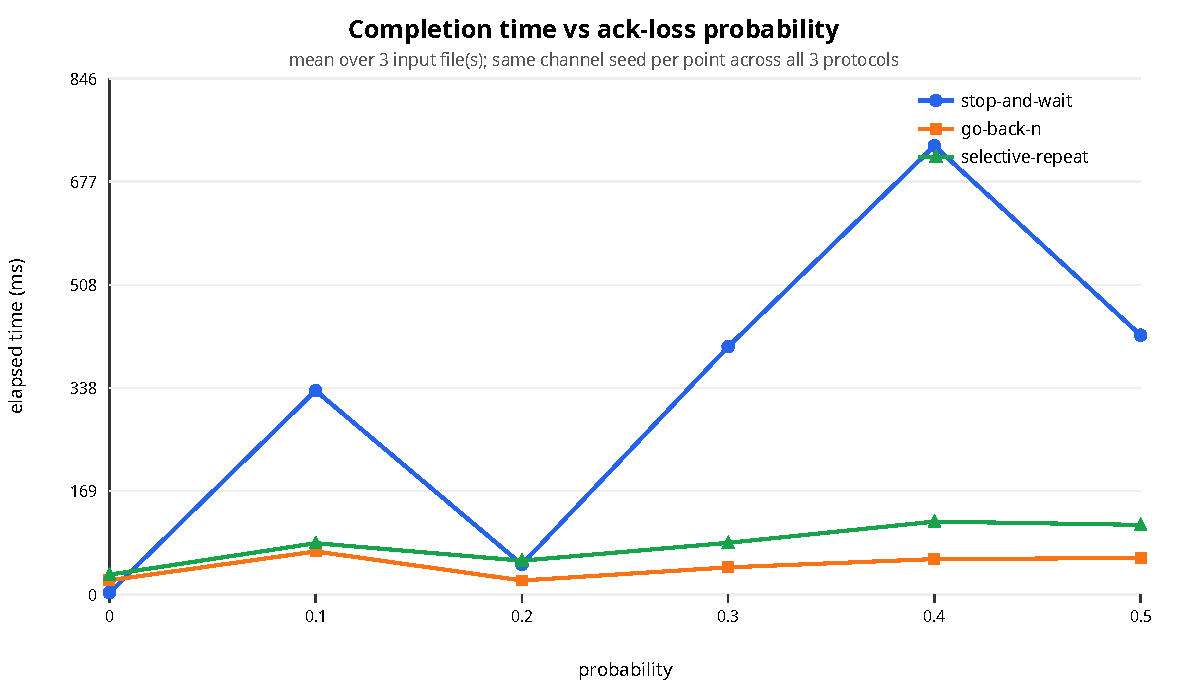
\includegraphics[width=0.85\textwidth]{figures/completion_ms_vs_probability_ack-loss.pdf}
    \caption{Completion time vs.\ ACK-path loss probability.}
\end{figure}

\begin{figure}[htbp]
    \centering
    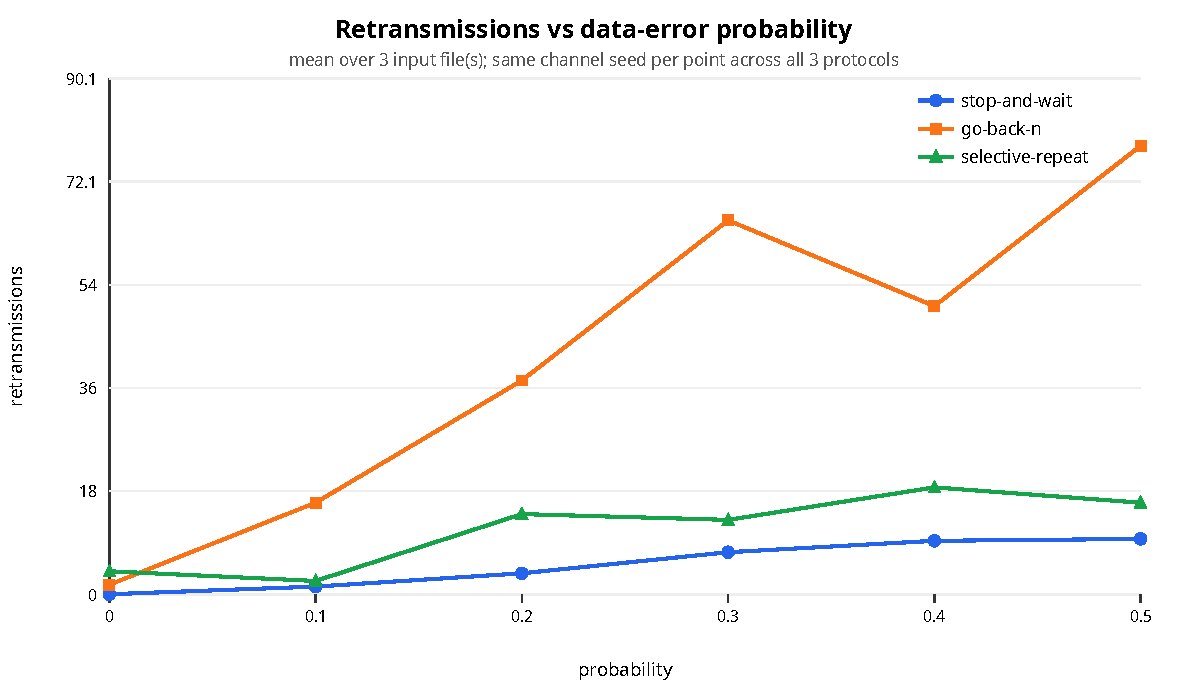
\includegraphics[width=0.85\textwidth]{figures/retransmissions_vs_probability_data-error.pdf}
    \caption{Retransmissions vs.\ DATA-path bit-error probability.}
\end{figure}

\begin{figure}[htbp]
    \centering
    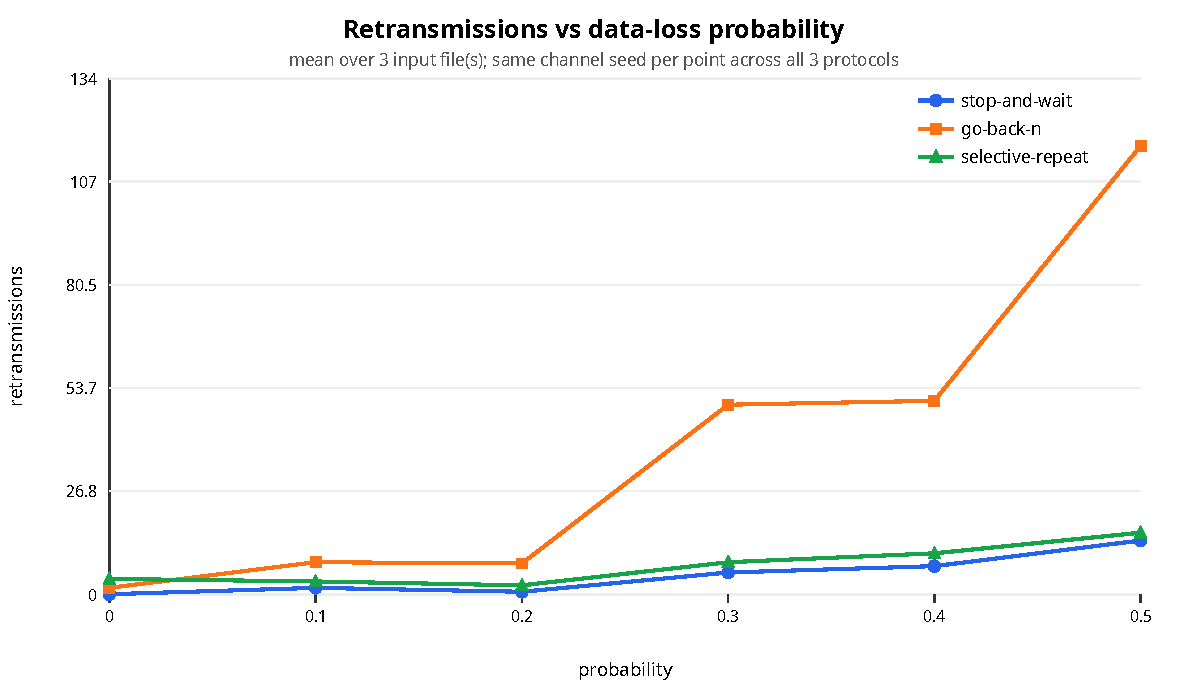
\includegraphics[width=0.85\textwidth]{figures/retransmissions_vs_probability_data-loss.pdf}
    \caption{Retransmissions vs.\ DATA-path loss probability.}
\end{figure}

\begin{figure}[htbp]
    \centering
    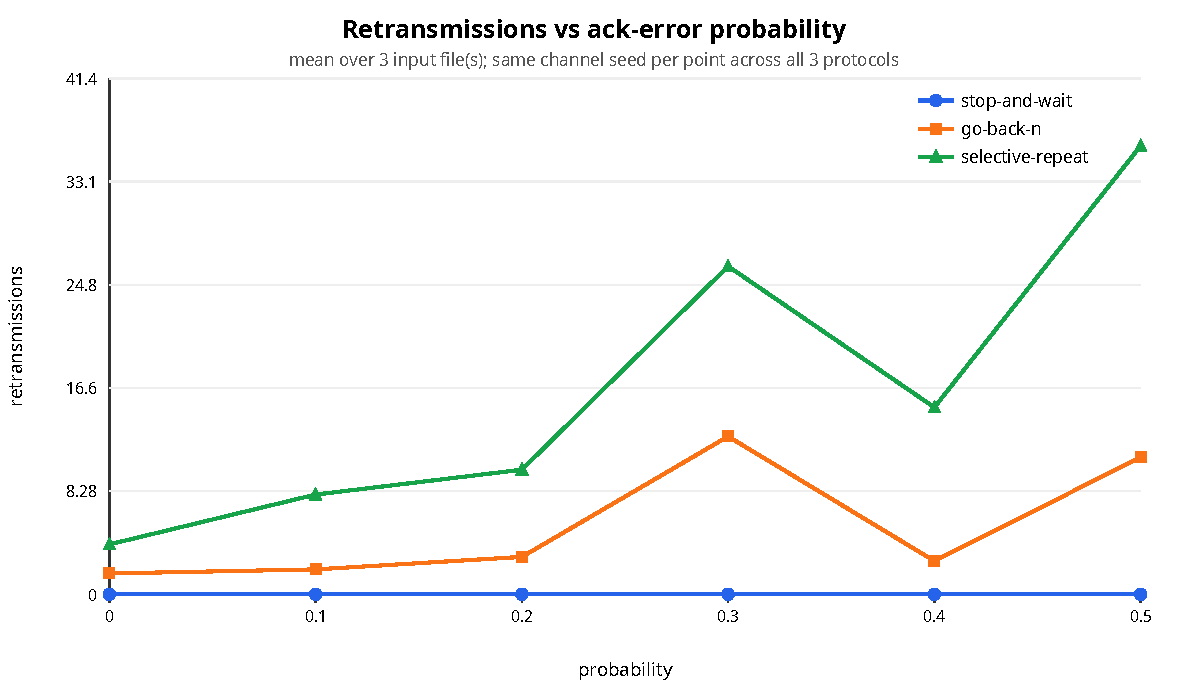
\includegraphics[width=0.85\textwidth]{figures/retransmissions_vs_probability_ack-error.pdf}
    \caption{Retransmissions vs.\ ACK-path bit-error probability.}
\end{figure}

\begin{figure}[htbp]
    \centering
    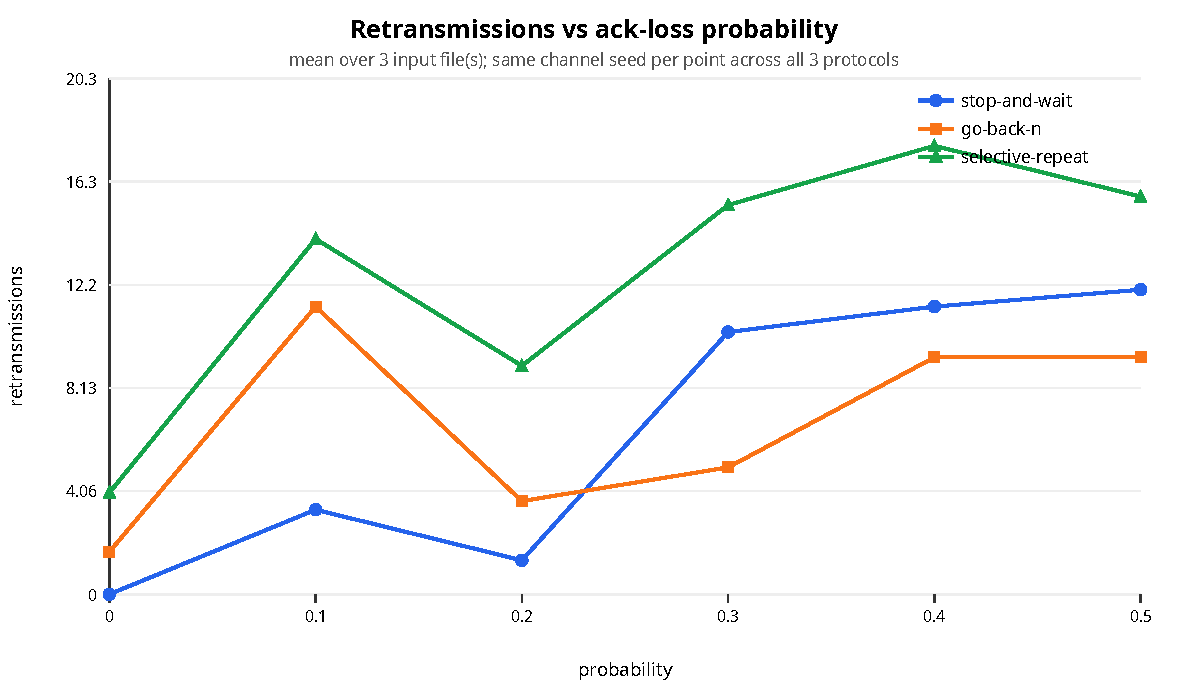
\includegraphics[width=0.85\textwidth]{figures/retransmissions_vs_probability_ack-loss.pdf}
    \caption{Retransmissions vs.\ ACK-path loss probability.}
\end{figure}

\begin{figure}[htbp]
    \centering
    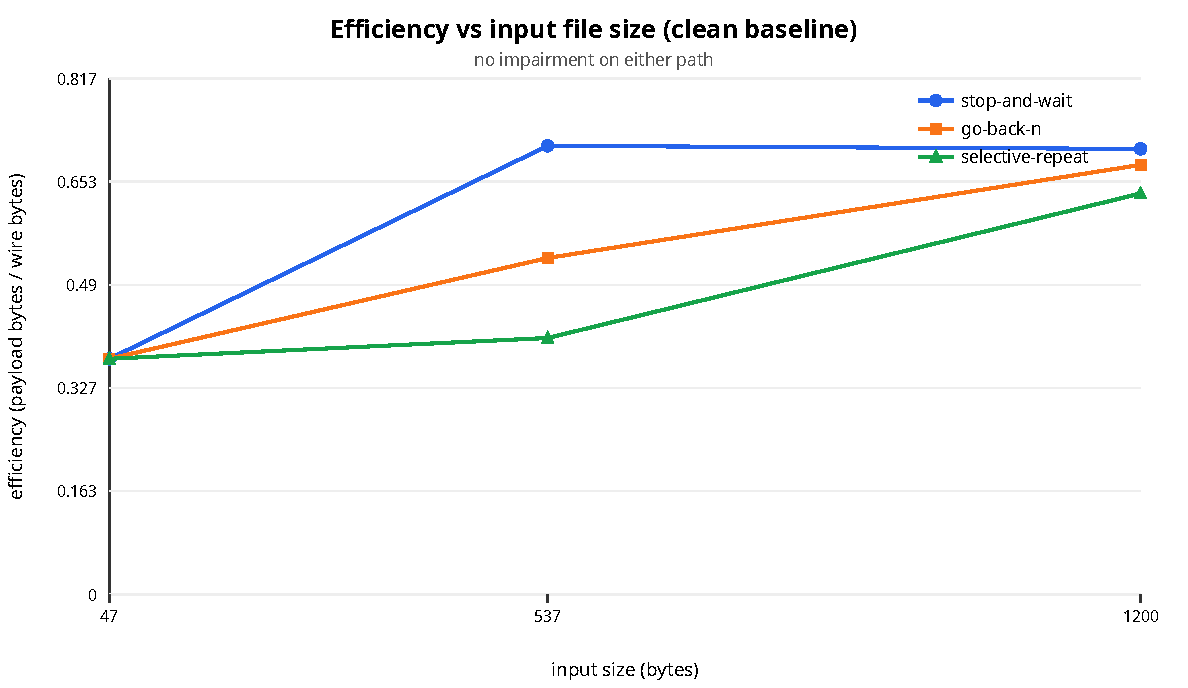
\includegraphics[width=0.85\textwidth]{figures/efficiency_vs_input_size_baseline.pdf}
    \caption{Efficiency vs.\ input file size at the clean baseline (no impairment on either path).}
\end{figure}

\subsection{Completion time}
{\sloppy
    Only wall-clock elapsed time is reported here; this implementation does not instrument
    sender/receiver CPU time or peak resident set size (see Known Limitations, Section 5.4).
    Completion time at the clean baseline is dominated less by protocol logic than by the
    real-timing effect discussed next: Stop-and-Wait's baseline mean of 2.476\,ms is noticeably faster
    than Go-Back-N's 22.881\,ms or Selective Repeat's 32.025\,ms, driven by the spurious timeouts
    those two protocols occasionally incur even at zero configured impairment.
    \par}

\section{Analysis}

\subsection{Correctness}
Every one of the \NumRuns{} automated matrix runs, plus the additional manual clean, impaired, and
edge-case runs described in Section 3.1, reproduced its input byte-for-byte. No run in this campaign
produced a mismatched output file.

\subsection{Protocol behavior}
Go-Back-N is the most sensitive to DATA-path impairment (Figure 1): because its receiver discards
any out-of-order frame, a single corrupted or lost frame invalidates every frame already sent behind
it in the window, and a timeout retransmits the \emph{entire} outstanding window rather than just the
missing frame. Selective Repeat avoids this cost by buffering valid out-of-order frames and
retransmitting only the specific frame that failed, which is visible as consistently higher efficiency
than Go-Back-N under DATA-path impairment at the same probability (Table in Section 4.3).
Stop-and-Wait, with its window forced to 1, has no window to invalidate and degrades the most
predictably of the three.

\subsection{Real-timing characteristic at the clean baseline}
A genuine, worth-flagging finding from this campaign: even with 0\% configured impairment,
Go-Back-N and Selective Repeat show measurable retransmissions and reduced efficiency on the
larger input files (Table in Section 4.2; Figure 13). Every one of those runs still verified
byte-identical, so this is not a correctness defect. It follows directly from Section 2.6's design
choice to use real \texttt{steady\_clock} timing via \texttt{SO\_RCVTIMEO} rather than a
deterministic simulated clock: under ordinary system scheduling jitter, a receive can occasionally
time out just before an ACK that was already in flight is read. Go-Back-N's whole-window
retransmission policy (Section 5.2) then amplifies one such spurious timeout into up to
\WindowSize{} retransmitted frames, while Stop-and-Wait (window 1) barely shows the effect. This
characteristic should be kept in mind when reading efficiency figures at low probabilities as purely
protocol-driven; some of the DATA-path-error curves' non-zero starting point at $p=0$ in Figures
1--12 is this effect, not injected error.

\subsection{Known limitations and bugs}
\begin{itemize}[nosep]
    \item Timing is real wall-clock time, not a deterministic logical clock (Section 5.3); results are
          statistically similar but not bit-for-bit reproducible run to run for the same seed.
    \item No CPU time or peak resident set size instrumentation was performed.
    \item A single fixed FCS scheme (CRC-16) and a single fixed payload size (46 bytes) are used,
          rather than an interchangeable scheme and a configurable payload range.
    \item No formal unit test executables exist for this implementation; correctness was established by
          the targeted manual runs in Section 3.1 and by the automated matrix's byte-identical requirement
          on all \NumRuns{} runs, not by an assertion-based test suite.
    \item \texttt{Channel::apply} draws both the loss decision and the corruption decision/position from
          one shared random-number generator per direction per run, rather than separately seeded
          selection and bit-position streams.
    \item Two bugs (Section 3.1) were found and fixed during the development of the experiment
          tooling itself; both are resolved as of this report, but are recorded here in the interest of
          applying the same rigor to this report's own verification process that it applies elsewhere.
\end{itemize}

\subsection{Possible improvements}
\begin{itemize}[nosep]
    \item Replace the plain EWMA timeout estimator with the full Jacobson SRTT/RTTVAR estimator
          and Karn's rule, to reduce sensitivity to the real-timing effect described in Section 5.3.
    \item Instrument sender/receiver CPU time and peak resident set size.
    \item Support a configurable payload size and an interchangeable FCS scheme.
    \item Record per-frame identities in the experiment output to support exact paired-frame analysis
          across protocols.
    \item Automatically generate the narrative sections from \texttt{results/experiments.csv} as well
          as the tables and figures, rather than hand-authoring the surrounding prose used here.
\end{itemize}

\section{Comments and Learning Reflection}
Choosing to fix the payload size and FCS scheme, and to accept real wall-clock timing instead of a
simulated logical clock, made the cost/benefit trade-offs of scope unusually visible: those choices
removed a great deal of implementation complexity, but that same simplification is exactly what
produced the spurious baseline retransmissions documented in Section 5.3 --- a direct, traceable
consequence of one specific design decision, not an accident. The two bugs found during the development of the
experiment tooling (Section 3.1) were both genuinely instructive: the stray-ACK race only appeared
under real timing pressure that a purely logical simulation would never have exposed, and the
seed-overflow bug was a reminder that a value generated in one language (Python's 32-bit
unsigned CRC) is not automatically safe to hand to another (C++'s signed \texttt{int} via
\texttt{std::stoi}) without checking the range explicitly.

\section{Conclusion}
This basic implementation meets its scoped goals: three working ARQ flow-control protocols over a
TCP carrier with an independently configurable, reproducible DATA/ACK channel simulation, and an
automated \NumRuns{}-run one-factor-at-a-time experiment matrix across \NumInputs{} input files,
every run verified byte-identical. The results match the expected theoretical trade-off between the
three protocols --- Go-Back-N's whole-window retransmission cost under DATA-path errors versus
Selective Repeat's more graceful, per-frame degradation --- while also surfacing and documenting a
genuine characteristic of this implementation's real-clock timing model rather than presenting the
results as if that characteristic did not exist.

\end{document}
